\documentclass[14.5pt]{article}
\usepackage{fancyhdr}
\usepackage{listings}
\usepackage{amsmath}
\usepackage{graphicx}
\graphicspath{ {./images/} }
\pagestyle{fancy}

\lhead{Samuel Petit 17333946 petits@tcd.ie}
\rhead{Statistical Methods Final Exam}
\renewcommand{\headrulewidth}{0.4pt}
\renewcommand{\footrulewidth}{0.4pt}

\begin{document}
\section*{Question 1}


\subsection*{Part a}
We have a total of 10 topics and need to pick 3, thus the amount of possible combinations
is $\begin{pmatrix} 10 \\ 3 \end{pmatrix} = 120$.


\subsection*{Part b}
To find an expression for the probability that none of the n topics studied come up,
I first find an expression for the opposite. That is at least 1 of the topics studied
come up in the exam.
To find that expression, I use the amount of combinations possible for 3 topics drawn out
of 10. I then need to find the amount of combinations such that one or more questions out
of n studied come up. This comes down to: $\begin{pmatrix} n \\ 3 \end{pmatrix}$.
Thus, the probability that one or more questions studied come up in the exam is:
\begin{equation}
    \frac{\begin{pmatrix} n \\ 3 \end{pmatrix}}{\begin{pmatrix} 10 \\ 3 \end{pmatrix}}
\end{equation}
We are looking for the opposite thus the probability that none of the n studied topics come up is:
\begin{equation}
    1 - \frac{\begin{pmatrix} n \\ 3 \end{pmatrix}}{\begin{pmatrix} 10 \\ 3 \end{pmatrix}}
\end{equation}


\subsection*{Part c}
Knowing that the above expression gives us the probability such that no topic out of the n studied
will be in the exam, we can derive it to include two scenarios.
The first one being that all of the topics on the exam were studied. To do this we take
the number of possible combinations of topics out of the ones studied, this is
$\begin{pmatrix} n \\ 3 \end{pmatrix}$. Please not that in the case that n is less than 3,
then $\begin{pmatrix} n \\ 3 \end{pmatrix} = 0$.
To obtain the probability of this scenario happening, we divide it by the number of combinations
of exam topics that we calculated in part a: $\begin{pmatrix} 10 \\ 3 \end{pmatrix}$.

The second scenario to consider is when exactly 2 topics on the exam were studied for, to compute
this we take the number of combinations of n choose 2. And to get the number of permutations with
the 3rd non studied topic, we multiply it by $ 10 - n $

Thus this gives us the following expression for the probability of failing an exam given that n
topics were studied:
\begin{equation}
    1 - [ \frac{(10 - n) * \begin{pmatrix} n \\ 2 \end{pmatrix} + \begin{pmatrix} n \\ 3 \end{pmatrix}}{\begin{pmatrix} 10 \\ 3 \end{pmatrix}} ]
\end{equation}

We then obtain the following graph using code from appendix a.
\begin{center}
    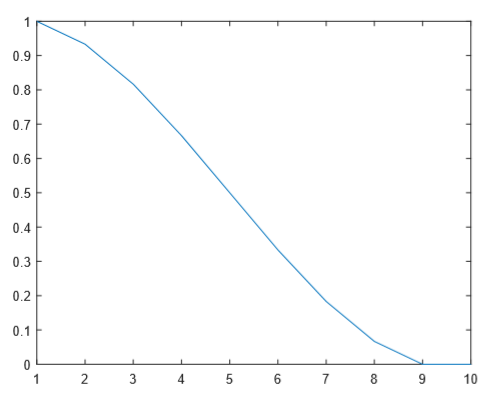
\includegraphics[scale=0.5]{p1}
\end{center}


\subsection*{Part d}
We can use the expression found in part d to come up with an expression for the same situation
where 4 questions are selected instead of 3.

We first notice that our scenarios change, we now have 3 different scenarios to consider in order
to find the probability of passing the exam, that is knowing 2, 3 and 4 topics from the exam.

For knowing 4 out of 4 topics, we use the same expression, changing 3s into 4s:
$\begin{pmatrix} n \\ 4 \end{pmatrix}$.
When 3 out of 4 topics were studied, we take the number of permutations for
$\begin{pmatrix} n \\ 3 \end{pmatrix}$ and multiply that by $10 - n $ the same way we did before
such as to get the total permutations including the 4th topic that was not studied for.
The final case, when 2 topics out of 4 were studied, we use the same principle as the latter, we
take the amount of permutations possible within these 2 topics and multiply it by the number
of permutations possible with the remaning $ 10 - n $ topics. This leaves us with:
$\begin{pmatrix} 10 - n \\ 2 \end{pmatrix}\begin{pmatrix} n \\ 2 \end{pmatrix}$

We sum these 3 scenarios and divide by the total amount of permutations of 10 topics in a 4 questions
exam:
\begin{equation}
    \frac{\begin{pmatrix} 10 - n \\ 2 \end{pmatrix}\begin{pmatrix} n \\ 2 \end{pmatrix}
        + (10 - n)\begin{pmatrix} n \\ 3 \end{pmatrix} + \begin{pmatrix} n \\ 4 \end{pmatrix}}
    {\begin{pmatrix} 10 \\ 4 \end{pmatrix}}
\end{equation}

We then obtain the following graph using code from appendix b.
\begin{center}
    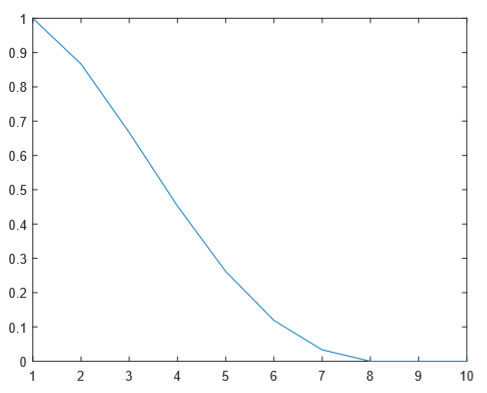
\includegraphics[scale=0.5]{p2}
\end{center}

Comparing this plot with the one from question c, we notice that for any equal amount
of topics studied, we have an overall higher change of passing with 4 topics in an exam
instead of 3. We also notice that the probability of passing becomes 1 at n = 8 instead of n = 9
for a an exam model containing 3 questions.

\subsection*{Part e}
The code for the stochastic simulation of the exam setup with three questions is
appended to this document in appendix c.
Please note that it is the function called \textbf{simulation3Questions} and that it
\textbf{may be used in the following questions}.


\subsection*{Part f}
The code for the extended simulation from part e, such that it runs the simulation
N times and returns the empirical mean is appended in appendix d.
Please note that it is the function called \textbf{simulationEmpiricalMean} and that it
\textbf{may be used in the following questions}.
Let's now compute the confidence intervals using the central limit theorem when
$ n = 7 $ with $ N = 1000 $ and $ N = 10000 $

We first need the mean and the variance thus we'll start by computing
$E[X_{i}]$ and $var(X_{i})$. We've seen in part c that an expression for
\begin{equation*}
    1 - E[X_{i}] = 1 - [ \frac{(10 - n) * \begin{pmatrix} n \\ 2 \end{pmatrix} + \begin{pmatrix} n \\ 3 \end{pmatrix}}{\begin{pmatrix} 10 \\ 3 \end{pmatrix}}]
    \leftrightarrow
    E[X_{i}] = [ \frac{(10 - n) * \begin{pmatrix} n \\ 2 \end{pmatrix} + \begin{pmatrix} n \\ 3 \end{pmatrix}}{\begin{pmatrix} 10 \\ 3 \end{pmatrix}}]
\end{equation*}
Thus, with $ n = 7$, $ E[X_{i}] = 0.8167 $.
To compute the variance, since the $ Y_{i} $ are independent,
\begin{equation}
    var(\frac{1}{n} \sum_{i=1}^N Y_{i}) = \frac{1}{n^2} \sum_{i=1}^N var(Y_{i}) = \frac{var(Y_{i})}{n} = \sigma^2
\end{equation}
Thus, using the empirical mean $ E[X_{i}] = 0.8167 $ and the equation for the variance in a bernouilli distributed
random variable: $ var(X) = \sqrt{p * (1 - p)} $, can get the standard deviation $\sigma$.
\begin{equation}
    \sigma = \sqrt{\frac{E[X_{i}] * (1 - E[X_{i})}{N}} = \sqrt{\frac{0.8167 * 0.1833‬}{N}} = \sqrt{\frac{0.3869}{N}}
\end{equation}
Here we have $N = 1000$ and $N = 10000$, thus:
$\sigma_{N=1000} = 0.01967 \\$
$\sigma_{N=10000} = \frac{0.3869}{10000} = 0.00622$

The 95\% confidence interval using the CLT is then
\begin{equation}
    [\mu − 2\sigma, \mu +2\sigma]_{N=1000} = [0.77736‬, 0.85604]_{N=1000}
\end{equation}
\begin{equation}
    [\mu − 2\sigma, \mu +2\sigma]_{N=10000} = [0.80426, 0.82914]_{N=10000}
\end{equation}
\subsection*{Part g}

\section*{Appendix}
\subsection*{Section 0}
The code in the following sections may make use of the following function:
\textbf{customNChooseK}. It is a function which uses nchoosek when $ n >= k $.
If not then it will return 0. Matlab's default implementation of this situation is
to throw an error which is why I decided to write this helper function.
\begin{lstlisting}
function [m] = customNChooseK(n,k)
    if(n < k)
        m = 0;
    else
       m = nchoosek(n,k); 
    end
end
\end{lstlisting}

\subsection*{Section b - Question 1d}
\begin{lstlisting}
y1 = zeros([1 10]);
x1 = 1:10;
% Compute the probability for all values of n
for n = x1
    y1(n) = 1 - (((10-n)*
    (customNChooseK(n,3))/customNChooseK(10,4))+
    (customNChooseK(n,4)/customNChooseK(10,4)) + 
    (customNChooseK(10-n,2)*(customNChooseK(n,2)/
    customNChooseK(10,4))));
end
%plot(x1, y1);
\end{lstlisting}

\subsection*{Section a - Question 1c}
\begin{lstlisting}
y1 = zeros([1 10]);
x1 = 1:10;
% Compute the probability for all values of n
for n = x1
    y1(n) = 1 - 
        (((10-n)*
        (customNChooseK(n,2))/customNChooseK(10,3)) +
        (customNChooseK(n,3)/customNChooseK(10,3)));
end
plot(x1, y1);
\end{lstlisting}

\subsection*{Section b - Question 1d}
\begin{lstlisting}
y1 = zeros([1 10]);
x1 = 1:10;
% Compute the probability for all values of n
for n = x1
    y1(n) = 1 - (((10-n)*
    (customNChooseK(n,3))/customNChooseK(10,4))+
    (customNChooseK(n,4)/customNChooseK(10,4)) + 
    (customNChooseK(10-n,2)*(customNChooseK(n,2)/
    customNChooseK(10,4))));
end
%plot(x1, y1);
\end{lstlisting}

\subsection*{Section b - Question 1e}
\begin{lstlisting}
function [X] = simulation3Questions(n)
    % number of topics
    a=1:10;
    % questions drawn
    questions = randperm(numel(a),3);
    % draw for studied subjects
    studiedSubjects = randperm(numel(a),n); 
    
    % get common topics
    pos=intersect(questions, studiedSubjects);
    if(length(pos) >= 2)
        X = 1; 
    else 
        X =0;
    end
end    
\end{lstlisting}

\subsection*{Section b - Question 1f}
\begin{lstlisting}
function [X] = simulationEmpiricalMean(n, N)
    passCount = 0;
    for i = 1:N
        % number of topics
        a=1:10;
        % questions drawn
        questions = randperm(numel(a),3);
        % draw for studied subjects
        studiedSubjects = randperm(numel(a),n); 

        % get common topics
        pos=intersect(questions, studiedSubjects);
        if(length(pos) >= 2)
            passCount = passCount + 1;
        end 
    end
    
    X = passCount / N;
end  
\end{lstlisting}
\end{document}